The properties of various moir\'e superstructure are well described in literature and Hermann gives a comprehensive overview in his paper \cite{hermann_periodic_2012}. One can conclude the following: \label{section:moire}

If lattice constants are equal like in the case of a graphene bilayer, the needed lattice mismatch occurs due to a rotation of the two layers. A moir\'e is always present if an over layer shows a lattice mismatch with respect to the substrate. 

For \textbf{isotropically scaled over layers} (refer to figure \ref{fig:moire-pattern-scaled}) one can calculate the scaling factor $$p=\frac{R^{'}_{O1}}{R_{O1}}$$ which gives the size of the over layer lattice in units of the substrate lattice. The moir\'e pattern shows the same Bravais lattice type than the substrate\cite[10]{hermann_periodic_2012}. If moir\'e and ad layer lattice are aligned ($\alpha=0$\textdegree) the direction of moir\'e and substrate is aligned. If the over layer is isotropically scaled and not rotated, the period of the moir\'e calculates to $$a_{moir\'e}=\underbrace{\frac{p}{|p-1|}}_{\kappa}a_{substrate}$$. With $a_{moir\'e}$ and $a_{substrate}$ are experimentally available, the ad layer lattice can be calculated with high precision (usually one order of magnitude more accurate than direction measurement of its period).

For a \textbf{scaled and rotated over layer} (figure \ref{fig:moire-pattern-scaled-rotated}, the angle between substrate and moir\'e ($\gamma$[rad]) scales with the angle between over layer and substrate ($\alpha$[rad]) as $\alpha=(1-p)\gamma$.

For rotated and isotropically scaled over layers, one can determine the $\alpha$ and $p$ from experimental observables $\gamma$(moir\'e angle to substrate) and $\kappa$(scaling factor) through relations $ \tan(\alpha)=\frac{sin(\gamma)}{cos(\gamma)+\kappa}\qquad p=\frac{\kappa}{\sqrt{1+\kappa^2+2\kappa cos(\gamma)}}$


\begin{wrapfigure}{l}{4cm} \centering
	\subfigure[Isotropically scaled and aligned overlayer (gr/Pt(111): $p = 0.89$)]{
		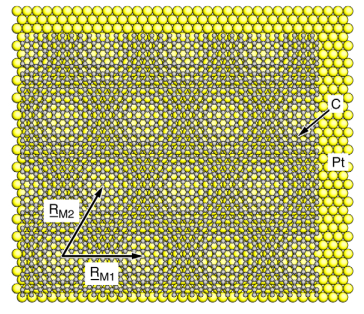
\includegraphics[width=0.25\textwidth]{./images/moire-scaled}%
		\label{fig:moire-pattern-scaled}
	}
	\subfigure[Isotropically scaled overlayer with rotation of \SI{5.4}{\degree} (gr/\textit{h}-BN: $p = 0.98$)]{
		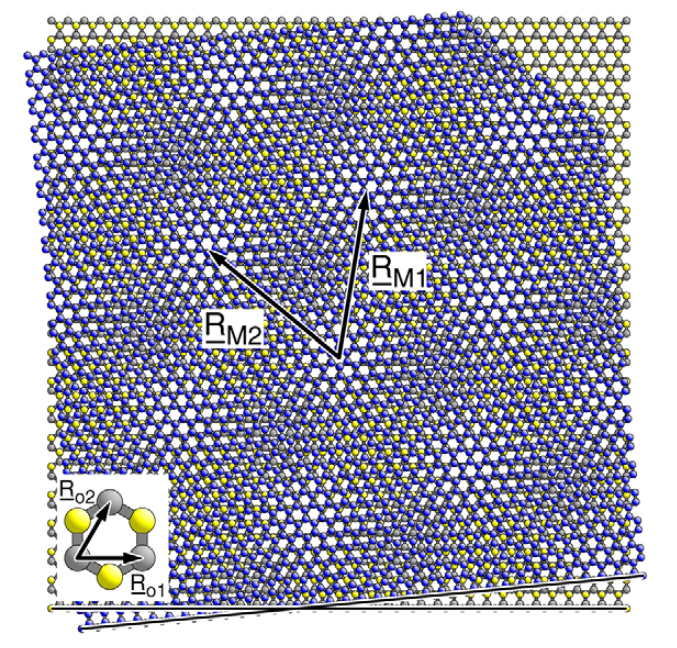
\includegraphics[width=0.25\textwidth]{./images/moire-scaled-rotated}%
		\label{fig:moire-pattern-scaled-rotated}
	}
	%	\subfigure[Isotropically scaled, alligned layer overgrowing a step edge (gr/Ir(111): $p = 0.91$)]{
	%		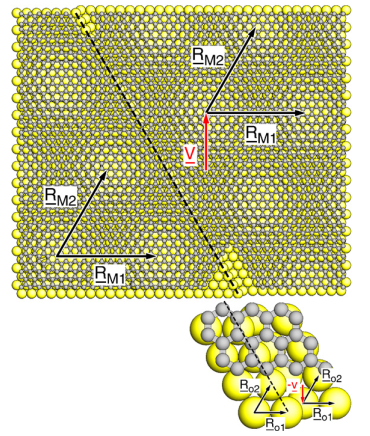
\includegraphics[width=0.25\textwidth]{./images/moire-scaled-step-edge}%
	%		\label{fig:moire-pattern-scaled-step-edge}
	%	}
	\caption{Adopted from \cite{hermann_periodic_2012}}
	\label{fig:moire-pattern}
\end{wrapfigure}\\

When a scaled over layers over grows a step edge, the moir\'e pattern is altered. While period and orientation remain the same, a lateral shift in the superstructure is observed that interrupts the regular pattern and shifts subsequent moir\'e features by a vector $\vec{V}$.

\begin{figure} \centering
	\subfigure[DFT simulation of \textit{h}-BN on Ir(111). The moir\'e unit cell as well as regions where B and N atoms occupy high-symmetry positions w.r.t. the Ir lattice are indicated. The change in adsorption height is caused by the changing registry of substrate (Ir) and ad layer atoms (B,N).  Adopted from \cite{schulz_epitaxial_2014}]{
		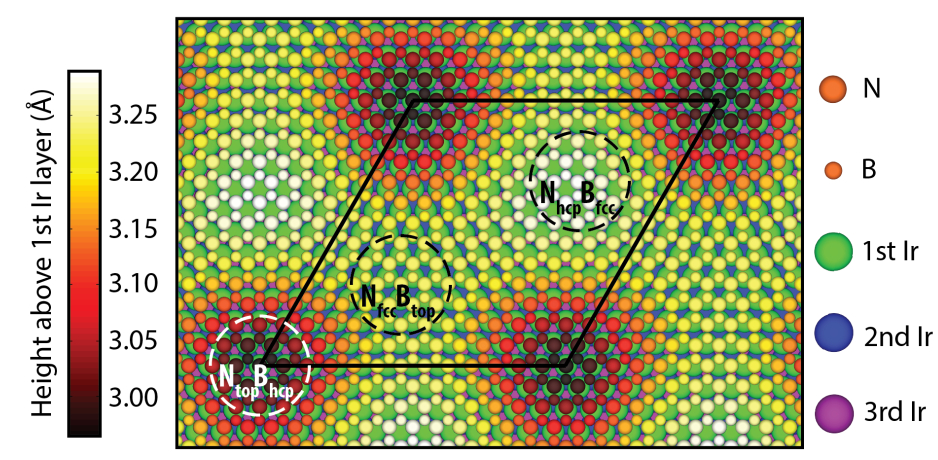
\includegraphics[width=0.5\textwidth]{./images/h-BN_Ir-moire}%
		\label{fig:h-BN-Ir-moire-DFT}
	} \quad
	\subfigure[\textbf{STM image of h-BN grown with CVD on Ir(111)}]{
		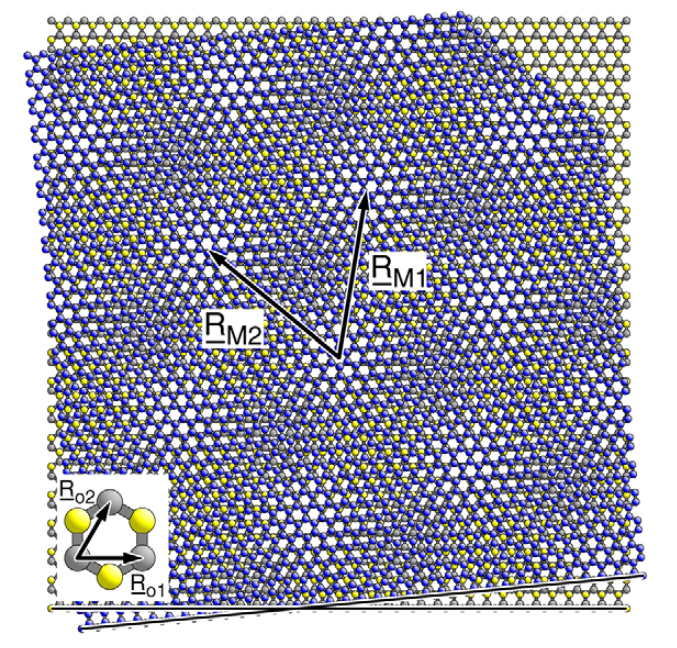
\includegraphics[width=0.25\textwidth]{./images/moire-scaled-rotated}%
		\label{fig:h-BN-Ir-moire-STM}
	}
	\caption{DTF calculation and STM images of \textit{h}-BN/Ir(111). While being aligned, a lattice mismatch creates a moir\'e  superstructure. It is well visible in adsorption height calculations \ref{fig:h-BN-Ir-moire-DFT} and as apparent height differences in STM images \ref{fig:h-BN-Ir-moire-STM}.}
	\label{fig:moire-DFT-TSM}
\end{figure}


\paragraph{Periodic change in work function}
A direct result of the lattice mismatch between \textit{h}-BN and substrate is the alternating registry of ad layer atoms and substrate. The periodic modulation of B/N registry to the substrate atoms results in regions of stronger and weaker interaction between \textit{h}-BN and substrate and is the reason for the nano templating effect of \textit{h}-BN on many substrates. 
In the following some resulting effects are discussed that lay the foundation for a nano patterning effect of \textit{h}-BN and its influence on the electronic structure of adsorbates.

After growth of h-BN the substrates work function in reduced [Rh: \SIrange{5.01}{3.07}{\eV} \cite{gomez_diaz_hexagonal_2013}. Therefor a dipole moment $\mu$ pointing from the the bulk to the surface is necessary \cite{roman_periodic_2013}, rather likely created by a negative charge transfer from the bulk into the ad layer.

\paragraph{\textit{h}-BN}
{% tex broke the page here!!!!
	\parfillskip=0pt
	\parskip=0pt
	\par}

Free standing \textit{h}-BN is investigated with \textit{ab-initio} calculations \cite{han_effects_2014,mortazavi_investigation_2012,topsakal_first-principles_2009,peng_mechanical_2012}. Together with experiments \cite{paszkowicz_lattice_2002} a crystal lattice constant of $a_{\textit{h}-BN, RT}=\SI{2.504}{\angstrom} $is derived. Depending on the substrates used, different lattice mismatches can be achieved as listed in \autoref{tab:h-BN-mismatch}. While substrates exist where the lattice constant are virtually identical ($\Delta \approx \leq \SI{1}{\percent}$), other substrates like Ag(111) show considerable deviations.

While a first report in 2004 \cite{corso_boron_2004}, pointed to the formation of a complicated two layer structure, later experiments \cite{roth_chemical_2013, li_grain_2015} including ours \cite{joshi_boron_2012, schwarz_corrugation_2017} and others  \textit{h}-BN/Cu(111) proposed a single layer of B \& N atoms in a regular hexagonal lattice. It evolved as well investigated system to perform experiments on. It could be shown that after CVD growth it adsorbs on Cu(111) as a flat layer. Due to its  lattice mismatch, "hill" regions  (corresponding to a $N_{top}B_{fcc}$ registry) and "valleys" (corresponding to a $N_{fcc}B_{hcp}$ registry) are formed. In these regions the work function is altered in opposite directions. While larger at the hill/pore regions, the work function reduces continuously to its lowest value in the valley/wire regions\footnote{Please note that the notation is not uniform throughout the literature. Sometimes hills are referred to as pores and valley regions are denoted as wire regions.}. 

With changing work function, a lateral electronic field emerges, pointing from \underline{\qquad \qquad}. It can be used to trap adsorbates with dipole moment along the field lines. This was shown for FePc and pentacene molecules on a graphene/Ru(0001) substrate. Here FePc molecules adsorp first on regions with high lateral dipole along top-fcc direction, followed by regions with lower lateral dipole. Pentacene molecules are trapped along the top-fcc direction \cite{zhang_assembly_2011}. This general adsorption mechanism is applicable for other systems with periodic modulation of the work function. \autoref{fig:ig:h-bn-cu-wf} depicts the work function change measured  with STM (Field emission resonances) indicating a similar modulation of the work function. In this theses TPB molecules (\autoref{section:TBP} and helicene molecules in \autoref{section:helicene} are used as sample molecules for specific adsorption site or orientation alignment.
\begin{wrapfigure}{r}{5cm}\centering
	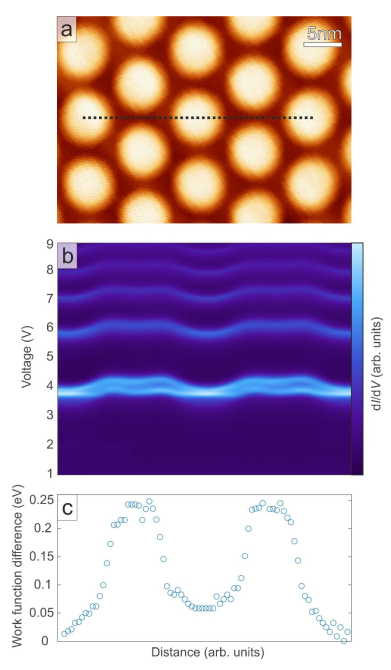
\includegraphics[width=5cm]{./images/h-BN-Cu(111)-wf-change}
	\caption{Work function variation along \textit{h}-BN/Cu(111) moir\'e. (a) STM image showing the \textit{h}-BN moir\'e with a periodicity of 8.4 nm. Scan parameter: $U_b= 4.0 V, I_t= 40 pA$. (b)	Field emission resonances acquired along the black dotted line in a) revealing a variation of the peak positions. (c) Work  function  differences  between bright  (“hill”/pore)  and  dark  (“valley”/wire)  regions obtained  from  the  dI/dV curves  of  the  field emission  resonances  displayed  in  b). Adopted from \cite{schwarz_corrugation_2017}}
	\label{fig:h-bn-cu-wf}
\end{wrapfigure}
\begin{table}\centering
\caption{Lattice mismatches between \textit{h}-BN and several transition metal surfaces. The mismatch is given to describe the relative size of the h-BN layer compared to the substrate, e.g. negative values indicate a larger lattice constant in the substrate bulk.}

	\begin{tabular}{ccc}
	Substrate 	& Mismatch [\%] \\ \hline
	Ni(111)		& \SI{+0.4}{\percent} \\
	Cu(111)		& \SI{-1.9}{\percent} \\	
	Rh(111)		& \SI{-7}{\percent} \\	
	Pd(111)		& \SI{-9}{\percent} \\
	Ag(111)		& \SI{-13}{\percent} \\

\end{tabular}
\label{tab:h-BN-mismatch}
\end{table}

As mentioned in \autoref{section:moire} the orientation of the moir\'e superstructure is determined by its rotation alone, while its period is determined by lattice mismatch, too. This results in a variety of moir\'e superstructure orientations and periods.



